
%%%%%%%%%%%%%%%%%%%%%%%%%%%%%%%%%%%%%%%%%%%%%%%%%%%%%%%%%%%%%%%%%%%%%%%%%%%%%

\newcommand{\reporttitle}{LogicAssistant}
\newcommand{\reportauthor}{Joshua Zeltser}
\newcommand{\supervisor}{Romain Barnoud}
\newcommand{\degreetype}{Computing}

%%%%%%%%%%%%%%%%%%%%%%%%%%%%%%%%%%%%%%%%%%%%%%%%%%%%%%%%%%%%%%%%%%%%%%%%%%%%%

% load some definitions and default packages
\documentclass[a4paper]{article}

%% Language and font encodings
\usepackage[english]{babel}
\usepackage[utf8x]{inputenc}
\usepackage[T1]{fontenc}
\usepackage{fitch}
\usepackage{bussproofs}
\include{thesis.preamble}
\usepackage{lipsum} % just for the example

\usepackage[nottoc,notlot,notlof]{tocbibind}
\newenvironment{bprooftree}
  {\leavevmode\hbox\bgroup}
  {\DisplayProof\egroup}


\usepackage{amssymb}
\usepackage{amsthm}
\theoremstyle{definition}
\newtheorem{exmp}{Example}[section]

\theoremstyle{definition}
\newtheorem{definition}{Definition}[section]
%% Sets page size and margins
\usepackage[a4paper,top=3cm,bottom=2cm,left=3cm,right=3cm,marginparwidth=1.75cm]{geometry}

%% Useful packages
\usepackage{amsmath}
\usepackage{graphicx}
\usepackage[colorinlistoftodos]{todonotes}
\usepackage[colorlinks=true, allcolors=blue]{hyperref}
\usepackage{tabto}

\newtheorem*{theorem}{Theorem}

% for specifying a name
\newtheorem{thm}{Theorem}[section] % the main one
\newtheorem{rules}[thm]{Rule}

\theoremstyle{plain} % just in case the style had changed
\newcommand{\thistheoremname}{}
\newtheorem{genericthm}{\thistheoremname}
\newenvironment{namedthm}[1]
  {\renewcommand{\thistheoremname}{#1}%
   \begin{genericthm}}
  {\end{genericthm}}

\setlength{\parskip}{1em}
\setlength{\parindent}{0pt}

\usepackage{pdfpages}

% load some macros
% Here, you can define your own macros. Some examples are given below.

\newcommand{\R}[0]{\mathds{R}} % real numbers
\newcommand{\Z}[0]{\mathds{Z}} % integers
\newcommand{\N}[0]{\mathds{N}} % natural numbers
\newcommand{\C}[0]{\mathds{C}} % complex numbers
\renewcommand{\vec}[1]{{\boldsymbol{{#1}}}} % vector
\newcommand{\mat}[1]{{\boldsymbol{{#1}}}} % matrix


\date{June 2017}


\begin{document}

% load title page
% Last modification: 2015-08-17 (Marc Deisenroth)
\begin{titlepage}

\newcommand{\HRule}{\rule{\linewidth}{0.5mm}} % Defines a new command for the horizontal lines, change thickness here


%----------------------------------------------------------------------------------------
%	LOGO SECTION
%----------------------------------------------------------------------------------------


\includegraphics[width = 4cm]{./figures/imperial}\\[0.5cm] 

\center % Center remainder of the page

%----------------------------------------------------------------------------------------
%	HEADING SECTIONS
%----------------------------------------------------------------------------------------

\textsc{\Large Imperial College London}\\[0.5cm] 
\textsc{\large Department of Computing}\\[0.5cm] 

%----------------------------------------------------------------------------------------
%	TITLE SECTION
%----------------------------------------------------------------------------------------

\HRule \\[0.4cm]
{ \huge \bfseries \reporttitle}\\ % Title of your document
\HRule \\[1.5cm]
 
%----------------------------------------------------------------------------------------
%	AUTHOR SECTION
%----------------------------------------------------------------------------------------

\begin{minipage}{0.4\textwidth}
\begin{flushleft} \large
\emph{Author:}\\
\reportauthor % Your name
\end{flushleft}
\end{minipage}
~
\begin{minipage}{0.4\textwidth}
\begin{flushright} \large
\emph{Supervisor:} \\
\supervisor % Supervisor's Name
\end{flushright}
\end{minipage}\\[4cm]

\includegraphics[width=90mm]{figures/imperial2}

%----------------------------------------------------------------------------------------
%	FOOTER & DATE SECTION
%----------------------------------------------------------------------------------------
\vfill % Fill the rest of the page with whitespace
Submitted in partial fulfillment of the requirements for the BEng degree in
\degreetype~of Imperial College London\\[0.5cm]

\makeatletter
\@date 
\makeatother


\end{titlepage}


\pagebreak
\tableofcontents
\pagebreak

\section{Introduction}

\subsection{Motivation}

Mathematical logic is an area used throughout the engineering and scientific industries. Whether its developing artificial intelligence software or students completing a Computer Science degree, logic is a fundamental tool. In order to ensure that logic is used correctly a proof system must be used. Natural Deduction provides the tools needed to deduce and prove the validity of logical problems, making it a vital tool for everyone to learn to use. This is why many universities make it a priority to teach this to their students as they begin their studies. For students new to Natural Deduction, or even those more advanced users, logicians are often left stuck in the middle of a proof not knowing what to do next, and then when they have completed the proof are unsure as to whether it is valid. LogicAssistant is being created to assist users with this problem.

Although the basics of Natural Deduction are easy to learn by just committing to memory the various rules that are defined, when it comes to more complex proofs it can be difficult to work out whether your proof is correct. You may have made an assumption at some point in your proof that was invalid, or just mistakenly used the wrong rule. It is not always the case that you can find someone who is an expert in this field who can check over your proof for you. This problem assumes that you are even able to get to the point of completing your proof. Often you may just have to sit staring at a certain point in your proof unsure of what to do next. You could at this stage go through each rule and try to work out which fits best, but this is quite a short-sighted approach as you may be going off in the complete wrong direction. This is also quite time consuming. When using Natural Deduction in the real world there is not always someone around to point out which rule to use next. 

In order to remedy these problems, I have built LogicAssistant which will contain a number of useful features that will aid users with their Natural Deduction proofs. The first feature which I aim to create is a proof checker which allows the user to type in their Natural Deduction Proof specifying all of the rules they have used, and the software will notify them to whether it is valid. I also want the user to be notified which parts of the proof are wrong and are thereby causing the proof to be invalid. This means that a user will never be unsure whether a proof they have created is valid and if it isn't they will know immediately where they went wrong. The other main feature that LogicAssistant will have is the ability to ask for hints at any stage of a proof. This means that if a user is stuck at any point in their proof they can ask the software to provide them with the next rule to apply. This will be very helpful especially for students who are new to Natural Deduction proof techniques. All of these features and more will be condensed together into an easy to use web interface that a user can access whenever they need to check or solve a proof. 

There are tools already out there that assist you with Natural Deduction. Most of these tools are very complex and difficult to use, requiring a high level of technical and mathematical knowledge to understand them. This makes them often a waste of time to use on a simple Natural Deduction proof. There are also tools like Pandora\cite{pandora} which allows you to enter your Natural Deduction proof step by step and then tells you whether it is valid. The drawback of this software is that it only allows you to enter a step in the proof if it is valid. This means that the amount that can be learnt from this tool is limited as through trial and error you could eventually solve your proof without really knowing what you are doing. The problem that these tools are trying to solve is quite complex and difficult to solve. There are lots of different rules to consider at any part of the proof, and when it comes to generating hints there are often several different possible rules to use next. The motivation of LogicAssistant is therefore to fill in the gaps left by existing solvers, in order to help solve the difficult problem of automating the validation and assistance process for logicians solving Natural Deduction proofs.

\subsection{Objectives \label{objectives}}

When starting this project I came up with a number of objectives that I wanted to achieve. Over time some of these goals may have changed depending on the level of difficulty or ease that I experience during different parts of the project. The first and main objective of this project was to create an easy to use proof checker for Propositional Natural Deduction proofs. A tool that can be used by anyone to easily check whether their Natural Deduction proofs are valid and if not they will be notified as to whether they have gone wrong. Once this was complete my next objective was to add on top of this a hint option which offers the user a hint as to the next step when they are stuck at any part of the proof. These two goals combined will allow me to create a tool that doesn't just help people who are trying to solve Natural Deduction proofs, but also acts as a learning tool for anyone new to this area. By the end of this project almost anyone no matter what their knowledge of logical proofs, will be able to use this tool to help them learn how to successfully create valid Natural Deduction proofs.

In order to ensure that my project is as easy to use and as useful as possible I also added the following additional objectives that time allowing I would like to complete:
\begin{itemize}
\item Add proof checks for first order predicate logic Natural Deduction
\item Add hints for proofs using first order predicate logic
\item Add a more advanced algorithm for hint generation
\item Create an aesthetically pleasing user interface
\item Add the ability to save and load Natural Deduction proofs
\end{itemize}

\section{Background \label{Background}}

\subsection{Propositional Logic}

A Proposition is a statement of some alleged fact which must be either true or false, and not both \cite{ndBook}. This basic form of logical reasoning can be used to represent everyday scenarios that we may face. Although this system has issues when trying to represent time and context this system can be used to represent some quite complex systems.

\begin{exmp}A list of propositions that could be represented by Propositional Logic
\begin{itemize}
\item England is in Europe
\item Elephants are big
\item three is smaller than two
\item Mark smells because he is muddy
\end{itemize}
\end{exmp}

Throughout this report I will represent propositions using a capital letter or a word starting with a capital letter. I will also use a number of operators to represent logical statements:
\begin{itemize}
\item Logical Truth will be represented by $\top$
\item Logical False will be represented by $\bot$
\item A logical And will be represented by $\wedge$
\item A logical Or will be represented by $\vee$
\item A logical Not will be represented by $\neg$
\item A logical Implication will be represented by $\Rightarrow$
\item A logical Iff (if and only if) will be represented by $\Leftrightarrow$
\end{itemize}

Propositions can be grouped together to form sentences using these operators. This is how Propositional Logic is used to model real life scenarios made up of events represented by Propositions. The syntax and grammer of a sentence in Propositional Logic is defined in Figure 1.

\begin{figure}[!ht]
  \centering
  \makebox[\textwidth]{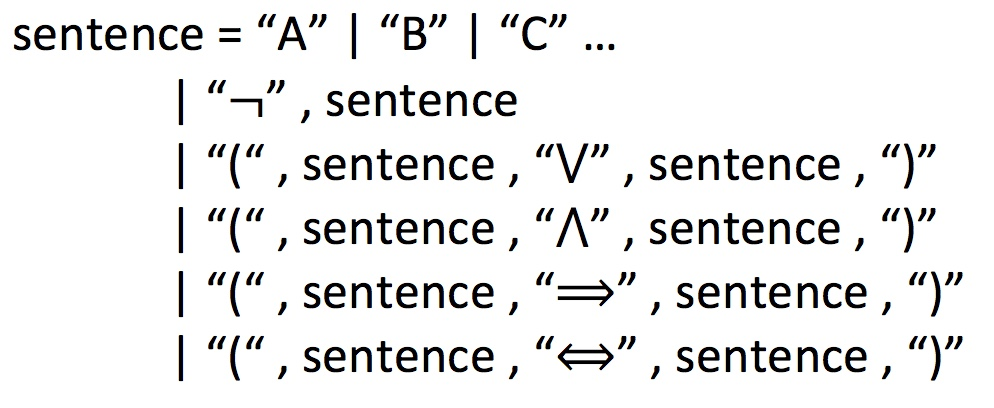
\includegraphics[width=100mm]{figures/PropositionalSentences}}
  \caption{Propositional Logic Grammar Rules}
\end{figure}

We have now defined a Propositional Logic language for this project. We have added brackets into our rules in order to ensure that we fully understand what a Propositional statement is saying and is therefore unambiguous. Without brackets some statements may become a bit ambiguous and difficult to understand. Truth tables can be used to interpret all of the possible results of a logical sentence. This helps users to plan for any possible outcomes of a set of propositions occurring.

\begin{exmp}Examples of Propositional Statements using our language
\begin{itemize}
\item A $\Rightarrow$ B
\item B $\wedge$ A
\item ((A $\Leftrightarrow$ B) $\vee$ C)
\item $\neg$A $\Rightarrow$ (B $\Rightarrow$ C)
\end{itemize}
\end{exmp}


\subsection{Predicate Logic}
Propositional logic is very useful when trying to represent the truth values of propositions, but there is limited scope in this formalisation as to the type of statements that can be represented. For example if I wanted to represent the statement "some boys like football", it would be very difficult to represent this using just Propositional Logic. This is why I decided to also check proofs of the more useful first order Predicate Logic. This logical system allows users to both apply properties to specific objects and add quantifiers to them. This makes it much more expressive and useful in real world applications. 

The properties that an object has is called a Predicate. Predicates can be unary where they have just one property, or they can be n-ary describing relationships between them and other predicates. Predicate logic also includes two quantifiers that allow this formalisation to be more expressive. The first quantifier is a "for all" quantifier ($\forall$). This allows us to represent statements like "all dragons are green". The other quantifier is the "exists" quantifier ($\exists$). This quantifier allows us to represent statements such as "some dragons are blue".These two quantifiers together, increase the expressive power we can create using this logical system. Below are some examples of statements that can be created using Predicate logic.

\begin{exmp}Examples of Predicate Statements
\begin{itemize}
\item $\forall x.P(x)$
\item $\exists y.bird(y)$
\item $\forall y.dark(y) \Rightarrow hates(x,y)$
\end{itemize}
\end{exmp}

\subsection{Natural Deduction}

The logical systems that were introduced above present a language and an interpretation using Propositional and Predicate atoms. All the reasoning that can be taken away from these systems are based on truth tables. Truth tables are a way of considering all of the possible outcomes of a statement filled with atoms that can be true or false. For simple systems truth tables are enough to be able to prove and reason about a situation. In order to be able to reason about much more complicated problems, the truth tables would be very large making it a time consuming problem to solve. We must therefore introduce a formal system which gives us the tools to solve and deduce these problems. To solve this problem Natural Deduction was created. Using a set of strict rules Natural Deduction allows us to deduce the consequences of any Propositional or Predicate statements we are given showing us the immediate outcome. This apparatus is very useful in solving logical problems in all areas. When a statement can be deduced from a number of premises using Natural Deduction we put it on the right side of a $\vdash$ symbol, while the original premises will be listed on the left of this symbol. Natural Deduction has a list of rules for both Propositional and Predicate logic allowing us to deduce the consequences of any premise. This proof solving methodology can also be used to solve proofs with no premises using its complex rule-set.

There are ten Propositional rules for Natural Deduction that can be used to form proofs (see Appendix \ref{appendix:nd-prop}). In this report I have outlined the rules based on the following process. Each rule consists of a horizontal line with the resulting expression or expressions placed beneath it. The expressions are either assumptions (where indicated) or expressions that need to be derived in order for the result below the line to be proven. For example, in the case of And Introduction, both A and B need to be derived in order for the introduction to come into affect. In several cases such as Implies Introduction, an assumption must be made and a sub-goal proven in order for the expression below the line to be proven. These rules can be combined together to make-up complex Natural Deduction proofs.

\subsubsection{Propositional Rules Examples}

Throughout this project I have used the Gentzen Natural Deduction system. This means that I lay out proofs as shown in the examples below. The first example shows a basic proof with the given premise written first followed by the various deductions made throughout the proof. On each line of the proof I write a justification of the rule that was used together with the lines that the rule has used to make the deduction.

\begin{exmp} Show that $A \wedge B \vdash A \vee B$

\begin{fitch}
\fj A \wedge B & Given \\
\fa A & $\wedge$-Elim (1) \\
\fa A \vee B & $\vee$-Intro (2) \\
\end{fitch}

\end{exmp}

The next two examples require an assumption to be made at some point in the proof that will allow the user to deduce their required outcome. Throughout this project when an assumption occurs in a proof I will highlight the assumption and its result by formatting it slightly to the right of the rest of the proof. This makes it stand out and more readable for the user, alerting them to the new scope that has been entered.

\begin{exmp} Show that $ A \Rightarrow B \vdash \neg (A \wedge \neg B)$

\begin{fitch}
\fj A \Rightarrow B & Given \\
\fr \fa A \wedge \neg B & Assumption \\
\fa \fa A & $\wedge$-Elim (2) \\
\fa \fa B  & $\Rightarrow$-Elim (1) \\
\fa \fa \neg B & $\wedge$-Elim (2) \\
\fa \fa \bot & $\neg$-Elim (4,5) \\
\fa \neg (A \wedge \neg B) & $\neg$-Intro (2,6)
\end{fitch}

\end{exmp}

\begin{exmp} Show that $A \Rightarrow B, B \Rightarrow C \vdash A \Rightarrow C$

\begin{fitch}
\fa A \Rightarrow B & Given \\
\fj B \Rightarrow C & Given\\
\fr \fa A & Assumption \\
\fa \fa B & $\Rightarrow$-Elim (1,3) \\
\fa \fa C & $\Rightarrow$-Elim (2,4) \\
\fa A \Rightarrow C & $\Rightarrow$-Intro (3-5)
\end{fitch}

\end{exmp}


\begin{exmp} Show that $A, A \Leftrightarrow B \vdash B$

\begin{fitch}
\fa A &  Given\\
\fj A \Leftrightarrow B & Given \\
\fa A \Rightarrow B & $\Leftrightarrow$-Elim (2) \\
\fa B & $\Rightarrow$-Elim (1,3) \\
\end{fitch}

\end{exmp}

The next example shows a proof which contains no premises but only the resulting expression. Several assumptions therefore have to be made using the Natural Deduction rules in order to solve this proof.

\begin{exmp} Show that $\vdash A \vee \neg A$
	
	\begin{fitch}
	
		\fr \fa \neg (A \vee \neg A) & Assumption \\
		\fr \fa \fa A & Assumption \\
		\fa \fa \fa A \vee \neg A & $\vee$-Intro (2) \\
		\fa \fa \fa \bot & $\neg$-Elim (1,3) \\
		\fa \fa \neg A & $\neg$-Intro (2,4)\\
		\fa \fa A \vee \neg A & $\vee$-Intro (5) \\
		\fa \fa \bot & $\neg$-Elim (1,6) \\
		\fa \neg \neg (A \vee \neg A) & $\neg$-Intro (1,7) \\
		\fa A \vee \neg A & $\neg \neg$-Elim (8)
	\end{fitch}
	
\end{exmp}

Although it is not an official rule, I have implemented an additional rule of availability to this project. This rule uses an already proven expression later on in the proof, in order to meet the desired outcome. This rule helps to keep proofs concise and readable, especially when it comes to more complex proofs. An example of how this rule is used can be seen in the example below:

\begin{exmp} Show that $B \vdash A \Rightarrow B$
	
	\begin{fitch}
		\fj B & Given \\
		\fr \fa A & Assumption \\
		\fa \fa B & Available (1) \\
		\fa A \Rightarrow B & $\Rightarrow$-Intro (2,3) \\
	\end{fitch}
	
\end{exmp}


\subsubsection{Predicate Rules Examples}

In Predicate Logic, similar Natural Deduction proofs can be created. These proofs, as well as using the Propositional rules, have their own set of rules (see Appendix \ref{appendix:nd-pred}) that the user can use to form a proof. This means that very complex proofs can be created. Below are some examples of what these proofs may look like.

\begin{exmp} Show that $P(m),  \forall x.(P(x) \Rightarrow Q(x)) \vdash Q(m)$

\begin{fitch}
\fa \forall x.(P(x) \Rightarrow Q(x)) & Given\\
\fj P(m) & Given\\
\fa P(m) \Rightarrow Q(m) & $\forall$-Elim (1) \\
\fa Q(m) & $\Rightarrow$-Elim (2,3) \\
\end{fitch}

\end{exmp}

\begin{exmp} Show that $\forall x. \forall y.P(x,y) \Rightarrow \neg P(y,x) \vdash \forall x.\neg P(x,x)$

\begin{fitch}
\fj \forall x. \forall y.P(x,y) \Rightarrow \neg P(y,x) & Given\\
\fa \forall y. P(a,y) \Rightarrow \neg P(y,a) & $\forall$-Elim (1) \\
\fa P(a,a) \Rightarrow \neg P(a,a) & $\forall$-Elim (2) \\
\fr \fa P(a,a) & Assumption \\
\fa \fa \neg P(a,a) & $\Rightarrow$-Elim (3,4) \\
\fa \fa \bot & $\neg$-Elim (4,5) \\
\fa \neg P(a,a) & $\neg$-Intro (4,5) \\
\fa \forall x.\neg P(x,x) & $\forall$-Intro (6)
\end{fitch}

\end{exmp}

\begin{exmp} Show that $s=t \vdash (s = u) \Rightarrow (t = u)$

\begin{fitch}
\fj s = t & Given\\
\fr \fa s = u & Assumption \\
\fa \fa t = u & Substitution (1,2) \\
\fa (s = u) \Rightarrow (t = u) & $\Rightarrow$-Intro (2,3) \\

\end{fitch}

\end{exmp}
\pagebreak

\section{Design}

The design methodology that I decided to use for this project is the Model View Controller architecture. This entails the separation of the front end website components from the back-end where the actual core functionality of the system is written. These two areas are then controlled by various controller classes, which bring all of these components together to create the finished application. I chose this methodology in order to make the system easier to understand and later build on. Whenever I need to add an extra feature to the application, I am able to just update the model part of the code-base and then change the front-end view code. This is much simpler than having all of the code together in one large code base. This methodology therefore made the development of this application much easier.


\subsection{Model}
In order to create the functionality required for me to meet my objectives, I had to come up with a fitting design that allowed lots of different tasks to work together. This often meant creating a Java Object with the sole use of solving one of the problems I set out to achieve. I tried to separate the different parts of my code base into obvious classes which would make the code easy to read for any third party.

\subsubsection{Component}
In both Propositional and First Order Predicate logics, logical expressions can be made up of two different components, Propositions (or Predicates for Predicate logic) and Operators. For this project both of these components require some common functionality such as how they are converted to Strings, how they are interpreted when input by the user and how equality between them is worked out. Due to this common functionality I decided to create an interface called Component which encompasses all the commonly used methods used by each of these components. I then created a Proposition and an Operator class which would each represent a component type. Each of these classes would inherit from the Component interface. This set-up was very useful in other parts of the code base as it allows me to pass in a Component and then check which type of component I am dealing with.  

The Proposition class, as well as inheriting and implementing the common toString and equals methods from the Components interface, contains functionality to set and retrieve the name of a Proposition. A Proposition is made up of a String field which represents the name of the Proposition. This is one of the main components of expressions that are used in this logical system.

The Operator class is used to represent one of the seven operators used in this logical system, as described in the Background section above (see \ref{Background}). This class also inherits the toString and equals methods from Components, making it much easier to use when building expressions. Each Operator object is made of a string which represents its name and an enum value corresponding to each operator. I have created an enum called OperatorType, which contains all of the different operator types used in this logical environment. The reason that I set operators up in this way is that it easily allows me to check what operator is being used in an expression at any time due to its uniquely identified enum value. The rest of this class is filled with getters and setters that help with the general functionality of this logical system. Here is a diagram of how this part of the code base is set up:

\begin{figure}[!ht]
	\centering
	\makebox[\textwidth]{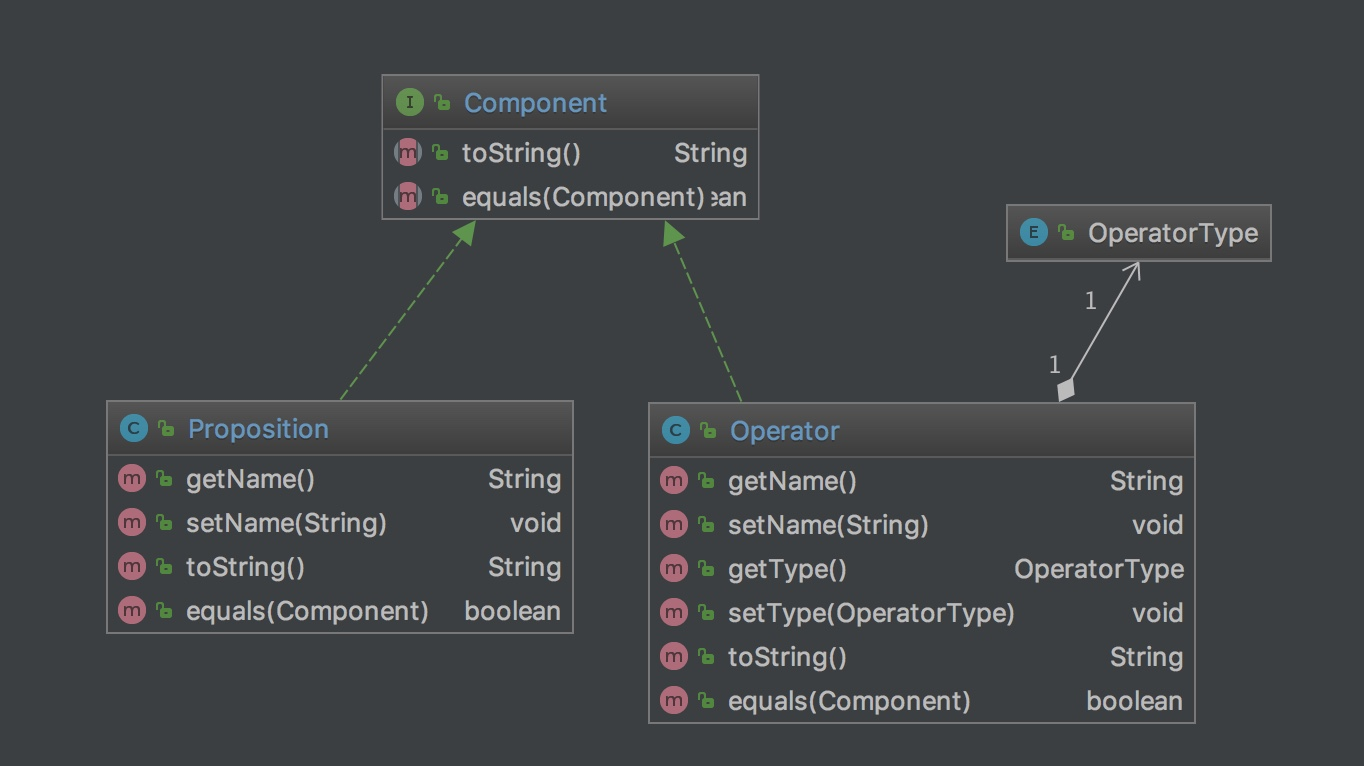
\includegraphics[width=\linewidth]{figures/ComponentsUML}}
	\caption{Component class structure}
\end{figure}

\subsubsection{Expression}

When using Natural Deduction, a proof is represented by a set of expressions each derived from previous expressions based on the Natural Deduction rule set (see Appendix \ref{appendix:nd}). I therefore created an Expression class which was made up of a number of parts. Firstly, each expression contains a list of Components making up the expression itself in terms of propositions and operators. An expression also keeps track of its line number in a proof. This is very useful when applying rules that depend on several different lines in a proof. Another key component of an expression is what rule was used to derive it. I therefore created a ruleType enum which enumerates all of the different rule types used in a natural deduction proof. This enum includes rules for premises and assumptions. This makes it very easy for the user to find out what rule was used when an expression is formed. This enum was also very useful when carrying out the proof validity checking process.

The most important functionality that the Expression class carries out, is the parsing of expressions from their String inputs. When a user enters an expression into the front end of the programme,  the expression is immediately tokenised by spaces and then each token is checked to see which type of Component it is. While this tokenization is occurring, the expression is checked for any syntax errors that may be present. If one is found, the entire process is halted and the syntax error that has occurred is outputted to the user. The tokens are then added to the list of components to make up the expression list. This process allows us to create an internal representation of the expression, making it easier to use when applying the various types of functionality used later on in the programme. 

In order to carry out the tokenization correctly, and to help with the various operations that are carried out on the expression throughout the code-base, a lot of extra functionality has been added to the Expression class. For example an equals method that allows the comparison of two expressions, and a contains method which allows a user to check whether a certain component is used inside a given expression. This functionality makes it easy to manipulate expressions as they are used to solve complex proofs. One really commonly used function that is implemented in this class is the splitExpressionBy function. This function takes an expression and splits it by the specified operator (assuming it contains this operator). This functionality is very useful when applying the various Natural Deduction rules to an expression, especially for elimination rules which require an expression to be split into one or two sub-expressions around this specified operator. The Expression class is therefore a fundamental building block for logical proofs in this project.

\subsubsection{Proof}

In order to represent the proofs that the user inputs into the system, I created a Proof class. This class contains a large amount of functionality used to represent these proofs in a way that they can be manipulated to help solve Natural Deduction proofs. In this class a proof is represented by a list of expressions, each representing a line in the proof. 

In order to populate a Proof object based on user input, this class reads in expressions and their associated rules and tokenizes them accordingly. It then fills the list of expressions in order to create the proof representation. While this is being carried out the code checks that each expression has been created using the specified rule correctly. For example if an expression was created using And Introduction, the code would check to ensure that both the right and left hand sides of the And operator have been proven earlier on in the code. If a rule has been used incorrectly, or cannot be used at this stage in the proof, then a rule error will be thrown aborting this entire process. Once all of the steps of the proof have been checked and been proven to have used the rules correctly the process will complete. This completion indicates that the proof so far is valid. 

When a user inputs each line of their proof along with the rule used, they also must include the lines that this rule used to create this expression.The software therefore must, when reading in this information, check that the lines mentioned are valid and correspond to expressions that can be used for this rule. As a proof is represented by a list of expressions it is easy to traverse the list and find the required expression by line number. Another additional complexity that has to be taken into account here, is the scope that the current expression is in. Whenever an assumption is made a new scope (or box), is opened until it is closed by certain rules being completed. Once this has happened nothing after the scope can use any expressions inside this scope for any further steps of the proof (apart from the result of the scope). This is another check that the code must make when checking whether a rule has been used correctly at any point of the proof. The Proof object is therefore what this project's main functionality is carried out on.

\subsubsection{Error Checking}

One of the main goals that I set at the beginning of this project, was to make a Natural Deduction solver which is a tool that can help teach people how to successfully solve these types of problems. I therefore made sure to have a very detailed error message system that allows a user to see exactly where they have gone wrong. This would mean that they can learn from any mistakes that they may have made. In order to make this as easy as possible, every error message that is displayed contains the type of error that has occurred, the line that it was thrown on as well as some extra information about the associated problem. This makes it very easy for the user to immediately understand what they have done wrong. In the case where no errors are thrown, the programme will display the string "Proof is Valid", alerting the user to their valid proof. 

The first type of error check that occurs as soon as the parser starts to read the user input, is for Syntax errors. This check ensures that each Component is placed in a valid part of the expression, so that each expression is valid. For example if two operators are added to an expression in a row, this error will be thrown. Similarly, if there are any mismatched brackets in an expression, a syntax error will immediately be thrown. This type of error is fundamental as the syntax of the proof must be completely correct in order for the user to move onto actually solving the proof at hand. This check is done right at the beginning of the parsing process for this very reason.

The other type of error check which helps to make this an educational tool, is for Rule errors. Whenever a proof is entered by a user, there is a function in the Proof class which goes through the proof and ensures that each line is valid. It does this by going through the list of expressions (the proof), and checks whether the specified rule can be used in the proof at this point. It also checks that the lines referenced by this rule are valid and are not out of scope. If all of the rules used are used correctly then the user is notified that the proof is completely valid. If not the user will be alerted to the line and rule which was incorrectly used, helping them to learn from their mistake. In order to clearly show the user all of the rules that have been broken at the same time, the Proof class contains an error list. This list slowly builds up as the proof is checked, and is then displayed after this process is complete. I decided to allow this accumulation of errors so that a user can fix several errors that exist at a time, rather than having to solve several over a long chain of trial and error. These error checks are done after any syntax errors, that may cause expressions to be invalid, have been fixed.

\subsubsection{Validity Checking}
Natural Deduction proofs can be quite long, adding an extra difficulty when trying to debug a mistake that was made in a proof. When solving a proof, it would be helpful to know that you can solve the proof with the given premises and result at all. It would be pointless to just start solving the proof if you will never reach the resulting expression. This is a major problem faced by even the more experienced solvers of these problems.

In order to remedy this potential issue I have added an optional extra validation stage before the main solver functionality. This stage allows the user to input their desired premises and result, and they will be used to check whether a proof using these expressions is valid. In order to implement this I have used the Truth Table validation method. This works by calculating the truth values of each premise and the result. The method then looks to see whether in the cases where all of the premises evaluate to true, the result expression also evaluates to true. If this is true for every case of the premises all evaluating to true, then we know that the proof is valid and that there is a possible proof that can be used to solve it. I implemented this check by first creating a TruthTable object, which is represented by a 2D array. When the user submits their premises and result, this array is populated with the possible input values for each proposition, the truth values of each premise in each of the cases, and the truth value of the result in each case. This object then has functionality that checks whether all of the truth values evaluate to true in the required cases, and if so designates this proof as valid. This whole mechanism will save a user a lot of time by allowing them to see immediately whether a proof they are about to try to solve is solvable.

\subsubsection{Hints \label{hints}}

One of the advanced features that I set out to implement during this project is hints. I wanted to allow a user to start a proof and if they become stuck at any step, they could use my software to gain a hint as to what rule to apply next. This feature is something that is lacking in similar software such as Pandora. When first planning to include this feature in the project,  I felt that I would start by implementing a simple form of hints, where when a hint was requested I would try each of the rules and reply to the user with any rules that didn't throw any errors. Obviously, this is quite a short-sighted way of implementing this as a user could be sent off in a completely wrong direction. Also when it comes to introduction rules there can be quite a lot of different possible cases to consider. I therefore decided that this methodology for generating hints is not useful for a user and started to explore some alternative methods.

Based on this exploration, I decided that the best way to implement this feature would be to actually apply an algorithm which solves the proof first. This would mean that when a hint is requested the system compares the users proof so far to the solved proof, in order to generate a hint for the next step. The first algorithm that I tried was one which took the premises that were given by the user and firstly tries each of the elimination rules on them several times. As this was happening the algorithm built up a list of possible proofs based on the steps found to be valid so far. The algorithm then tried some introduction rules in order to move further into the proof. This process would continue in a loop until either the resulting expression was reached, or a time-out was met. I also added a few enhancements to the algorithm that meant right at the beginning the algorithm looked at the resulting expression to see whether it, for example, contained an implications operator, meaning that an assumption needed to be added to the proof in order to form part of the implies introduction rule. Although this algorithm was able to solve the proofs in order for hints to be generated, in proofs which include any introduction rules, the algorithm took quite a long time. In some cases that I tested, a proof took over thirty seconds to be solved. This is due to the large number of options that needed to be tried for each introduction rule, adding even more possible combinations to the list of possible proofs. Obviously, this algorithm would not be able to scale very well. I therefore decided to search for some more efficient algorithms to use to solve this problem.

After much research, I found a very effective proof solving algorithm in a paper called Automated First Order Natural Deduction \cite{ndAlgo}.  This algorithm works in a completely different way to the one I devised above. The algorithm creates two lists, the first of which is called list\_proof containing the steps of the proof that have been solved at any point in the algorithms execution. The algorithm also includes another list called list\_goal, which contains the goal of the whole proof, as well as any sub-goals that are created through any introduction or the Or elimination rule. The algorithm works by first adding the premise, if there are any, to the list\_proof list and the resulting expression to list\_goal. It then tries out each of the elimination rules to see if they can be applied at this point of the proof. If one is found to be valid, it will be applied and the resulting expression is added to list\_proof. Then when each elimination rule has been checked, the algorithm moves onto the introduction rules. If it finds one of these introduction rules as being a valid step in the proof it will add the newly introduced equation to list\_goal, in order for the algorithm to work out a way to reach this new sub-goal. If appropriate, the algorithm will at this point add an assumption to list\_proof. After this the algorithm will start checking elimination rules again until this sub-goal is met. Once all of the sub-goals and the main goal itself are met, the algorithm adds this last goal to list\_proof. list\_proof now contains the completed proof that can be used for hints. The main benefit of this algorithm, is that by setting up sub-goals, the algorithm does not have to spend large amounts of time looking for possible combinations of expressions for introduction rules. Rather it knows the goal of the introduction rule and will apply the appropriate rules in order to meet it. This algorithm therefore works quickly in all cases and can scale very well. This makes this algorithm very efficient and is why I chose to use it for this part of my project. 

In addition to the basic algorithm, I added a few features to optimise the speed that the algorithm runs at. In particular at the start of the algorithm I added a check which looks at the resulting expression of the proof and sees from the start whether it contains an implication operator or starts with a not operator. If so then the algorithm now knows that the last rule applied will either be implies or not introduction. The algorithm can therefore skip the elimination rule checks at the beginning and go straight to these introductions. This speeds up the whole process in these cases significantly. The paper that I retrieved this algorithm from defines its Or elimination rule slightly differently to how I do in this project. For this project in order to carry out an Or elimination, I split the two sides of the Or operator into two separate boxes and try to find the same resulting expression in each, thereby eliminating the original expression. I therefore had to add some extra functionality for this case into the algorithm. This works by me adding the assumption of the left hand side expression to list\_proof and adding the assumption of the right hand side expression to another temporary list. I then continue with the algorithm as normal, but use both lists at each step. Then when both list\_proof and the temporary list have reached the same conclusion, I add the contents of the temporary list to list\_proof and then add the concluding step for the Or elimination rule. By implementing this rule in this way, I am able to use my definition for this rule whilst still benefiting from the use of this efficient algorithm. Using this algorithm I am able to solve any proof, and based on this provide the user with hints at any stage of a proof to help them learn how to solve Natural Deduction problems. 

In order to make this part of the software as useful to the user as possible, I decided to add two advanced extensions. Firstly, it is now not just at the end of a proof that a user can ask for a hint, but also in the middle. Sometimes when solving a natural deduction problem you can work out some sub-goals that will appear later on in the proof by working backwards from the goal. However, you may not be able to work out how to get to this sub-goal. In order to help combat this problem I have adapted the hint algorithm to allow the user to leave gaps in the middle of the proofs, and when the proof is submitted, hints will be generated to fill these gaps. This feature is really important as a good technique to use when solving these proofs by hand is to work backwards, and now it is possible to continue using this method even when you get stuck, through the use of hints. The second advanced feature that I have added is the tailoring of hints towards how the user has input the proof. Often there are multiple ways to solve a proof using Natural Deduction. The solving algorithm that this software uses tries to find the shortest optimal solution for these proofs, but that doesn't mean that other longer methods are invalid. As this is a learning tool, I decided that the hints generated should try to, where possible, follow the route that the user has started to take. Even if this means a longer proof, at least the user will be learning how to create valid proofs; the main objective of this tool. I added this by injecting the parts of the proof that the user has already input, into the algorithm. This means the algorithm continues to function based on this input, helping to tailor the generated proof and thereby hints to the users method. These two extra features together make this programme an invaluable tool when learning to solve these complex problems. 

\subsection{View}

One of the key components of this project is the design of the front-end. I wanted to make the application as easy to use and as appealing as possible to users looking for help in solving their Natural Deduction proofs. I therefore spent a long time perfecting this part of the application. As mentioned below (see \ref{JavaSpring}), I used Java Spring to create a front end that uses the Java back-end of this project. This meant using Thymeleaf together with HTML and Javascript to create an easy to use, but powerful user interface. In order to perfect the website I carried out several iterations before deciding on this final design.

The website itself is made up of three pages. The first of which is the home page, which contains most of the core functionality of the application. This page is made up of several different components. When you load the page the first part you see is the two text areas right in the middle of the page. The left one includes line numbers and allows the user to type in each step of their proof. The text area on the right allows the user to add a rule for each line of their proof. A key is conveniently displayed on the left hand side of the page, to show the user how to represent each of the operators in this logical system. In order to insert a rule corresponding to a line in the proof, on the right hand side of the page there is a list of buttons each representing a different rule. When one is clicked on that rule is added to the next line of the proof. If the rule needs references added to it regarding the lines in the proof it is using, the user can type these into the text area manually. If an assumption is used at any point of the proof, this left text area will automatically indent itself to represent any boxes (scopes) included in the proof. Once the user has completed their proof they can click the submit button towards the bottom of the page, and the solver will alert them to whether their proof is valid. If not, it will display any syntax or rule errors, including some extra helpful information to assist them in solving any issues that may be present. If the user becomes stuck at any part of their proof, they can click the "Hint" button at the bottom of the page so that it turns green. This means that hint mode has been turned on, so that when submit is now clicked, a hint will be delivered to the user in the output box at the bottom. If the hint button is used after the proof has already been solved, the user will be notified to this fact. Also, as mentioned above if the user has lines in the middle of the proof that they are stuck on, they can leave a blank line and an associated hint will be generated. All of these front end features together make up the main functionality of this programme.

This page also contains some other features that assist a user when using this software. Firstly, there is a drop-down menu towards the bottom of the page, that contains two useful options. An option to reset the page in order to type a new proof, and also a save proof as option. This allows the user to save any proofs they have, so that they can be revisited again on a later occasion. On the left hand side of the page there is also functionality that allows the user to upload their own proofs. This programme has its own file type (.la) and files of this type can be uploaded to this solver. The proof then can either be checked or added to and then saved again for future use. All of these small features together make using this system much simpler and straightforward for users to use.

The next page of the web-app is the proof validation page. This can be accessed using a button on the left hand side of the home page. This page allows the user to type in their chosen premises and the resulting expression that they want to use in their proof. Then by clicking the "Check Validity" button, the validity algorithm will be triggered alerting the user as to whether the proof will be valid. This step saves the user a lot of time by allowing them to see whether the proof they are about to solve is solvable before they even start the proof solving process. Once this check has been completed the user can navigate back to the home page in order to actually solve their proof step by step.

The final and most important page of the application is the User Guide. This page contains a detailed analysis of how to use all of the features mentioned above. With the help of this page I believe that almost any user will be able to work out how to use most of the functionality on the website. In addition to this, throughout the website I have added tooltips onto some of the key pieces of functionality. This means that when a user puts their mouse over one of these tooltips they will be shown a small speech bubble explaining what that piece of functionality is used for. This will increase the ease at which new users are able to benefit from this software. This is therefore how the front end (or view) part of my application has been created.

\subsection{Controller}

In order to coordinate and control the model and view parts of this web-app, it was necessary to add some controller classes. As I used the Java Spring framework to build this application (see \ref{JavaSpring}), I was provided with some special controller functionality that can be used to control the entire programme. Therefore, each page has its own controller class which retrieves a mapping based on the url, and allows the passing of Java objects into the front end of the application. For example the main page receives a mapping of "/", as it is the home page, and the controller passes in a Proof object so that the associated functionality can be applied. This controller also has a post mapping which returns to this same page after the form has been submitted. Similarly, the validity page has its own controller which receives a mapping of "/validity" as the browser enters that page. The controller then provides a TruthTable object to the front end, so that it can be used to carry out the validation checks. These two controllers are therefore really important as they allow the various pages to communicate with each other, as well as to the back-end of the programme. This therefore completes the set up of the Model View Controller infrastructure that I have built for this application.

\section{Development Tools}

\subsection{Java}

When embarking on a project such as this, the language that is chosen to implement all of the complex functionality is very important. In particular the chosen language must be compatible with front-end infrastructures. Lots of languages also have extra features such as large testing frameworks and advanced IDE's that would make the whole process of making an application much easier. Also once a language has been chosen it would be a lot of work to then transfer to another language. I therefore spent quite a long period of time deciding which language was best suited for this project.

The first language that I considered using was Prolog. Prolog is already a language based on logical systems, and had I used it, representing logical statements would have been much simpler. I also found a user interface library that uses Prolog itself to create a front-end website for applications. Based on these finds I could have built this application using Prolog. The main drawback for me of using this language, is that I am not as familiar at using it as other languages, meaning that I would have to waste a lot of time learning the language first before actually starting the application. Also, some of the more advanced features that I wanted to add, such as hints, would have been quite hard to implement using this language. I therefore in the end decided to look at other languages to use for this project. 

The language I ended up settling on for this project was Java for a number of reasons. Firstly, Java is the language that I am most familiar with and I am able to use many of its advanced features and large array of libraries. This made it very easy for me to create the representation of Proofs, as well as some of the more advanced functionality for this project. Another reason that I chose to use Java is the number of libraries and data structures it offers. I was able to use advanced lists and hashMaps throughout the code in order to ensure that all of the required functionality worked as efficiently as possible. Other languages like Prolog do not have these resources. Java also supports the use of the JUnit library (see \ref{JUnit}), allowing me to ensure that all pieces of functionality are working as expected through the creation of a large test suite. On top of all of this, there are lots of tips and references available for the Java language for me to use whenever I needed them. The only drawback that I found of using Java, is that it meant writing quite a large amount of code to create simple functionality, which can be quite time consuming. However, due to my knowledge of the language this did not hinder my progress too much. 


\subsection{Java Spring \label{JavaSpring}}

For this project, as I wanted to use Java to create the back-end functionality of the programme, I needed to find a framework that would make it easy for me to create a front-end that is compatible with this code. I also wanted to ensure that I was able to create a Model View Controller architecture for the code-base. I therefore decided to use the Java Spring framework to structure my project. Java Spring provides a Model View Controller architecture, including all of the components that I needed to create a web application. It allowed me to create my back end code in Java and then using Java Spring's controller functionality, I was able to connect it to the front-end part of the project. 

In order to be able to actually use the Java objects and functionality that I had created, in the front-end of the application, I was able to use Thymeleaf. Thymeleaf is a front-end technology compatible with Java Spring that allows the use of Java objects, as well as the calling of methods on these objects. This therefore made it very easy for me to add any back-end features to the front-end user interface. When I first started to use this technology there was quite a steep learning curve, as there are quite a lot of intricate details that must be adhered to in order for it to work. However, for the end result this technology turned out to be a very useful asset to this project. Thanks to me using this technology, I have been able to create a well structured project that is very easy to extend.


\subsection{Javascript}

In order to carry out a lot of the extra front-end functionality, such as uploading and saving files or controlling what each of the buttons does, I decided to use Javascript. Javascript is a very commonly used client-side language, that is compatible with HTML, which the web-pages are written in. Javascript made it relatively easy therefore, to add all of these important features to the user interface. 

\subsection{JUnit\label{JUnit}}

When carrying out large scale software projects such as this, one of the most important tasks that must be carried out is testing. There is no easy way to tell whether your code is completing the task you created it for without tests that put your code in realistic scenarios and see how they function. This is especially true for edge cases which in reality may never happen, but there is always the possibility. As I used Java for this project it was natural to use the very powerful JUnit test suite. JUnit allowed me to carry out individual unit tests on almost all of the functionality that I have created in the back-end of the application. Through the use of Test Driven Development (see \ref{TDD}), I was able to use the test suite itself to help me work out how to implement some of the more complicated code. This also allowed me to keep track and ensure that any new code I added wasn't breaking any other parts of the code-base. Using the JUnit assertTrue and assertFalse functionality, in each test case I was able to compare the computed result with the expected one, in order to ensure everything was working correctly. JUnit made this a smooth and easy process saving me a lot of time that I could dedicate instead to adding more features to the application.

\subsection{Selenium \label{selenium}}

When a project involves creating a front-end user interface in order to access its back-end components, it is important to ensure that all of its features are working properly. It is therefore not enough to just test the back-end of the application, but rather the front-end also needs to be tested. In order to carry this out I used Selenium together with the WebDriver tool, to create some front-end unit and integration tests. These tools enabled me to automate web application testing, by simulating user input into the various pieces of functionality on the web page. Then Selenium would check whether the behaviour that was caused by these interactions were as expected, and if not the tests would not pass. I created a large test-suite of these tests to ensure that the entire front-end code-base could be tested. I did not include these tests in my git-hook or Maven build, due to the large amount of time it takes to run them. However, they are still an invaluable tool to use to ensure everything is functioning properly throughout the code-base.

\subsection{Maven \label{maven}}

This project involved me using a combination of different technologies in order to create the finished product. In order for these tools to work together effectively I decided to use Maven. Maven allowed me to bundle together the Java Spring capabilities with the Java code and JUnit tests to create an efficiently functioning system. I was able to add dependencies for each of the tools to the Maven project, and through using the standard Maven directory set up, I was able to also add my front end code to this package. By using this containerisation I was able to easily deploy my application at any part of the development process to check that it was working correctly. Maven also allowed me to ensure that all of the JUnit and front end tests that I had set up were run before the programme was deployed, allowing me to make sure all parts of the code-base were functioning correctly. Maven also helped me to set-up other tools such as Github and Heroku for this project, with each of these tools being compatible with the Maven infrastructure.

\subsection{Intellij \label{intellij}}

When writing Java code it is very easy to make small syntactic mistakes in the code without realising. Whether its a missed semicolon or even the wrong number of curly brackets. This is especially poignant in larger code bases. The easiest way to avoid having to spend large amounts of time looking for these bugs and continually rerunning the code as you slowly fix them, is by using an IDE. There are many IDE's to choose from for the Java language, but I decided to use Intellij for a number of reasons. Firstly, Intellij has a very large range of features that would make coding this project much easier. For example on top of just alerting me to syntax errors, there is a code duplication error system, as well as built-in re-factoring functionality that allows me to make my code much more readable and efficient at the click of a button. On top of this, Intellij is compatible with Maven meaning that I can even build my Maven project inside Intellij, making the entire process much smoother. This compatibility goes so far that Intellij also downloads any dependencies that I have added to the Maven "pom" file. All of these reasons and more make Intellij the ideal IDE to use for this project.

\subsection{Git \label{git}}

A key area that needs to be considered when carrying out any large scale project such as this is version control. One cannot afford to lose their projects source code, and it is really useful to have previous versions of the code-base that can be returned to at any point in the project. For this project, I decided to use Git for this as I am very familiar with its functionality and so would be able to effectively utilise all of its useful features. In order to manage my git repository, I decided to use Github. Github has a really easy to use interface and is compatible with Maven making it very easy for me to upload my project. I was able to create a private project on Github and using its easy to use website I was able to look up previous versions of my code base whenever necessary. Github also provides some very useful statistics about how the version control side of my project is progressing. I used these statistics to try to keep up a good level of Software Engineering practise.

One git feature that was really useful for me throughout the project was the use of git hooks. I created a Git hook which whenever I commit my work, runs all of my unit tests over the code and ensures that they all pass. If any fail, the commit is halted and I must fix the associated errors before being able to commit. This is a very useful feature as often after changing one part of the code-base, you may accidentally break the code somewhere else. Without git hooks these errors may not be picked up on, meaning that broken code is committed to git.  This is obviously not a good technique to follow, so I made sure to add these hooks as early as possible in the project to avoid this from happening.

I structured my Git network by mainly working off a branch called backEnd. In general this branch contained the latest code that I was working on, whether or not it was fully functioning. When I decided to work solely on a single large task, such as hints, I would create a separate branch for this feature. Once this feature was completed and had been fully tested, I would merge it back into the backEnd branch. Every time I finished a large part of the front-end or back-end code-base and it was working with no test failures, I would merge the backEnd branch into master. This meant that the master branch always contained the latest, fully functional version of the project. This is why I used the master branch to deploy the project to Heroku (see \ref{heroku}). By using Git in this way,  if something went very wrong in the code-base I could always revert back to the fully working version that is saved onto the master branch of the project. Overall, through this set-up, I was able to successfully carry out this project without worrying about breaking or losing any of the already functioning code.

\subsection{Heroku\label{heroku}}
As my project is a web based application, I wanted to find an easy way to deploy it as a real website. Heroku allowed me to easily do this, as well as offering me many useful features. I was able to easily connect my Maven project to its services through my Github account, setting it up so that whenever I pushed my changes to master, my Heroku site would be updated. I therefore used my site on Heroku to house my latest fully functioning version of the app. This allowed me to show others and gain feedback on the parts of the functionality that I had already successfully created. Deploying my application in this way also allowed me to test it on other browsers and operating systems, to ensure that all of the required functionality functioned correctly. Once the project was completed, I permanently deployed the application to this free service for anyone to use.


\section{Project Management}

\subsection{Schedule \label{schedule}}

In order to ensure that I am able to meet the objectives that I set out at the beginning of this project, I created a project plan. This plan consists of seven iterations, each of which builds on the previous adding new features and fixing any discovered bugs. On top of these iterations I will also be regularly meeting with my supervisor to ensure that my progress is on track and heading in the right direction. The iterations have been made quite long periods of time in order to ensure that all of my tasks are completed to the best of my ability. The iteration lengths also take into account other university work that I may be working on concurrently with this project.The iterations are quite flexible so that tasks can be moved between iterations where necessary, to ensure that all the tasks are successfully completed. 


\subsubsection{Iteration 1 - 1/12/2016 $\Rightarrow$ 8/1/2017}

The first iteration involved completing the various tasks needed to set up and plan the project as a whole. Firstly, I plan to research the area of Natural Deduction as deeply as possible to ensure that I fully understand the rules and other technical terminology involved. This will allow me to envisage exactly what needs to be done to complete my objectives. Based on this research, I will next decide which features I want to add to the project and based on this decide which tools to use. I will decide which language is best suited for this project and which other tools are necessary to use that will help me fulfil my goals. Once tools have been chosen, I will set up version control and create a blank directory for this project. Next, I will plan my future iterations to ensure that all tasks can be completed in the short time frame I have. Throughout this iteration I will meet with my supervisor several times to ensure that all of my plans are feasible and on the right track.

\subsubsection{Iteration 2 - 9/1/2017 $\Rightarrow$ 10/2/2017}

For this iteration, I will start to actually code the first parts of the software for this project. To start with I will create a representation of Propositional logic that will be understood by the system, as well as a way to tokenise and convert string input into this representation. Next, a parser will be created that checks whether a rule that was parsed in is valid based on the Propositional Natural Deduction rules. On top of this, I will create a back end representation of a proof that can be checked using the parser. This completes a basic back-end that allows a user to enter a proof and each step in the proof will be checked to ensure that it abides by one of the Propositional Natural Deduction rules. Throughout the creation of the back-end part of this software, I will ensure to rigorously test all of the added features. This will ensure that the entire code-base at this stage is working, stopping bugs from occurring in future iterations. 

This iteration will not just involve me working on the back-end of this project, but also on the front-end. In order to be able to help test that my proof validity checker works completely, I will create a simple web interface that allows a user to enter a proof and click a "check proof" button. This button will then apply the back end functionality to check whether the proof is valid. By the end of this iteration my first objective will have been completed of creating a tool which allows a user to check whether their Natural Deduction proof is valid. As this is one of the core components of the project I have made the timespan of this iteration quite long to ensure that it is completed.

\subsubsection{Iteration 3 - 11/2/2017 $\Rightarrow$ 10/3/2017}

In this iteration I will focus firstly on completing the second of my main two objectives of creating a Natural Deduction proof checker with hints. At this stage, the functionality to check whether the proof that has been entered is valid has been completed, so can be used to work out which possible rules can be applied next by the user (hints). This functionality will allow the user to stop at any point in their proof and allow them to click the "Hint" button. The software will then produce a suggestion of which rule to apply next. This is quite a fundamental part of my project so I have given myself quite a lot of time to complete it, leaving time to test the code-base making sure that it is working correctly.

On top of adding this extra functionality, I also want to create a nice looking and easy to use user interface. Before this iteration I had only created a basic user interface which allows the user to type in their proof and then press various buttons to check whether their proof is valid. This however is not very intuitive to use and is not very nice to look at. In this iteration, I intend to add a HTML template to the interface to make it look much nicer and professional, as well as insert my back-end functionality into this template. This, as well as creating an aesthetically pleasing, interface ensures that my software is easy to use. By the end of this iteration I will have completed my main two objectives and thereby created a fully functioning and easy to use Natural Deduction proof checker for Propositional logic.

\subsubsection{Iteration 4 - 27/3/2017 $\Rightarrow$ 21/4/2017}

Up to this point, I have only focussed on Propositional logic and how Natural Deduction proofs using this logical system can be checked. However, this logical system is not very expressive and so is not usually used to model everyday situations. A much more useful logical system is first order Predicate Logic. In this iteration I want to firstly start creating a representation in my code for Predicate logic. This will be slightly harder to implement than for Propositional logic as it involves taking into account quantifiers, adding a complete other dimension onto this logical model. Once this basic Predicate representation has been created, I will start to add functionality that checks whether steps in Natural Deduction proof using this logical system are valid. This is very similar to how rule checking in the Propositional case was implemented,  as I will just be checking based on the set of Predicate logic rules for Natural Deduction. However, these rules are slightly more complicated to check for in a proof so I have allowed myself extra time to complete this task. 

As well as this major addition to the back-end of my project, I will also need to update the front-end accordingly. I will add some basic functionality that will allow me to user-test this new back-end functionality. This would probably just comprise of a dialogue box and a few buttons. This will give me enough functionality to test the new Predicate proofs to make sure they are valid. Overall, this iteration is slightly shorter than previous ones, but I now will be able to work on this project full time having finished my other commitments allowing me to focus fully on this project. 

\subsubsection{Iteration 5 - 22/4/2017 $\Rightarrow$ 12/5/2017}

In the last iteration we created a representation of Predicate logic together with a checker for Predicate Natural Deduction proofs. Now, as was implemented for Propositional logic, I will add hint functionality that the user can use while composing their proofs. As I have already created rule verification in the last iteration, this iteration includes the application of these rules to any step in the proof to give the user an idea of what to do next. This as with the Propositional logic part of this project is a very useful part of this tool. 

Now that we have completed the Predicate Logic part of the back-end of the project, I will make sure that the user interface is as user friendly and presentable as possible for when the user tries to use the Predicate parts of the tool. This may mean adding extra web pages and features to allow the user to choose between the types of logic they want to use in their proofs.

\subsubsection{Iteration 6 - 13/5/2017 $\Rightarrow$ 2/6/2017}

At this point, I have completed all of the main features of my Natural Deduction checking tool. There are however some other features which would be really useful for users, so this iteration allows some time to add these additions. One feature in particular that I would like to add at this stage is a more advanced hint system. At this point in the project although hints will have been implemented, they would be functioning by checking whether each rule can be used at a step and when the "Hint" button is pressed all possible rules are output. This is a very inefficient way of doing this and can lead to the users' proof going off in the completely wrong direction. At this stage of the project I therefore intend to employ a more advanced algorithm which actually solves the proofs in order for me to generate an accurate hint. This extension will be quite advanced and therefore time consuming, meaning that most of this iteration will be spent implementing this feature. However, if I am able to implement it, this tool will be invaluable to someone working through advanced Natural Deduction problems.

In this iteration I would also like to spend time adding some other extensions such as the saving and loading of proofs. This would allow the user to upload proofs that they have written elsewhere and also save any proofs they have now checked to use elsewhere. These extensions are all dependent on the amount of time I have left at the end of the project.

\subsubsection{Iteration 7 - 3/6/2017 $\Rightarrow$ 30/6/2017}

From the start of this iteration, I want to have stopped adding any new features. I will go through my code, tidy it up, add comments and ensure that all unnecessary code is removed. I will also look through and try to solve any remaining bugs left in my code-base. At the same time I will complete my report noting how the various parts of the project were carried out. I want to allow as much time as possible to do this, to make sure that I can create a high level and well written report. This iteration will also be used to create a presentation of the project making sure it looks professional and is able to inform the audience of exactly what my project can do.

\subsection{Testing \label{testing}}

In order to efficiently carry out a software project in any area, a fundamental programming tool to use is testing. By building large test suites that are able to cover most of the possible cases that the software will deal with, a programmer can ensure that their entire code-base is working to its full potential. I therefore spent a large amount of time on this component of my project.

\subsubsection{Test Driven Development}
From the outset of this project I realised how important testing would be for me as I carried out this project. I therefore decided to adopt the Test Driven Development methodology. This meant that before starting to create each feature a set of test-cases would be written that I would expect to pass once the functionality was complete. This created two main benefits. Firstly, I would know when the functionality that I am creating has been successfully finished, as these tests will now pass. On top of this, as new functionality is added, I was able to ensure that the rest of the code-base was still functioning properly and had not been broken. This system therefore made it very easy for me to add new features to the code-base. This methodology was mainly used in the back-end of the project, where it was easy to write large test suites using JUnit. In the end, by using this methodology a large test suite of over one hundred and ten tests was created. 

\subsubsection{Back-End}
The main parts of this projects functionality were created in the back-end of the code-base. As this was written in Java I was able to easily write large test suites using JUnit. As mentioned above (see \ref{maven}), Maven was used to package and deploy this project. By writing a large number of back-end test I was able to link my test-suites to my Maven build, ensuring that the code-base is fully working whenever the programme is deployed.

The large number of test cases that have been corrected for the back-end of this project, test lots of different areas of the code-base. I therefore split the test-cases into five different classes. The first test class I created tested the various operations that can be done on expressions. When I was creating the Expression class in the back-end, these tests enabled me to create Expressions which can be manipulated in the various ways that I would need to later on in the project. Next I created an error test class. One of the most important features of this software that makes it educational for the user, is the error messages that are produced when mistakes are made. There are lots of different possible error messages that could occur depending on the case that the user is in. I therefore made sure to write lots of tests which check to see that the correct error messages are being displayed at any time. This helped me to create this error message delivery system. 

The next and most important section of tests is for Natural Deduction rules. One of the key features of this software is the checking of Natural Deduction proofs to ensure that they are valid. In order to do this the software checks that each rule that is used in the proof is used correctly. This part of the project required a lot of code to be written so I had to ensure that no code was broken as new parts were added. I therefore created a test class just for the rules. This class contains twenty nine tests which go through all of the Natural Deduction rules and tries to ensure that the checks that are made are done so correctly. I also tried to add some edge cases which may have tricked the code that I had written to run these checks. With the help of this test class, I was able to be confident that this part of the project was functioning well.

The final and largest test class is for the solver and hint components of the project. The algorithm that I used to solve natural deduction proofs in order to generate hints (see \ref{hints}), has been proven to work in all cases. However, I had to make sure that the way I created it, with the extensions that I added worked just as well. I therefore created an in-depth test-suite to test both simple and more complex cases that this part of the software could be faced with. Due to the large number of possible cases, I had to create a high number of tests. This meant that I spent a long time perfecting this test-suite in order for it to be a useful tool for this part of the project. Overall, these test classes together helped me to perfect each part of this project, ensuring that it is able to work in almost any case that is thrown at it.

\subsubsection{Front-End}

A major component of this project is the front-end, which the users themselves will be using to access the useful functionality that this software provides. This part of the project is very important as the user will use this to judge how well the software solves their proof solving problems. It would therefore be wrong for me to just create test-cases for the back-end of the project. Therefore, using Selenium (see \ref{selenium}), I was able to create integration tests which actually act as the user by clicking on the buttons and typing in input. These tests allowed me to see how the user experiences the website itself, and whether each of the features works for them. Just because my features work in the back-end of the software, it does not necessarily mean that they will also work in the front-end. Therefore I must use these front-end tests to ensure that all parts of my software are functioning correctly. These tests were very useful after each feature was created to ensure that they were working as expected throughout the development process.

\subsection{Trello \label{trello}}

One of the hardest parts of any large software development projects, is managing the large list of tasks as the project progresses. As I am coding I am constantly thinking of new features or extensions that would improve the software, and it is very easy to forget to implement them later on in the project. I therefore needed a way to sort these tasks and ensure that none of them are forgotten. To solve this problem I decided to use Trello. Trello is a project management tool that allows you to create lists of tasks that you need to complete for your project. The lists can be customised using different colours and labels helping you to plan the devlopment process of your project. I have found this tool very useful in the past, so I decided to use it again for this project.

I set-up my Trello board by creating four different lists. I created a list for all of the back-end tasks that I would need to do, a list for all of my front-end tasks, a list of any bugs that I had found in the code-base and a list of completed tasks. This set-up allowed me to look through my back-end and front-end task lists to help me decide which tasks to complete at any point of the development process. Then once these tasks were completed I could move them to the "Completed Tasks" list. As I went through these tasks any additional tasks that I thought about could be added to the lists to be implemented later on. I was able to similarly do this with any bugs I found, stopping me from forgetting about them later on in the project. Another really useful feature that I used was labels. Whenever I thought a certain task in the project was very important, and it was necessary for me to implement it as soon as possible, I could label the task in red. This indicated to me that this task needed to be completed next. Overall, this tool really helped me to manage my work-flow as I went about developing this complex software. The image below shows my Trello board at one point in the development process.

\begin{figure}[!ht]
	\centering
	\makebox[\textwidth]{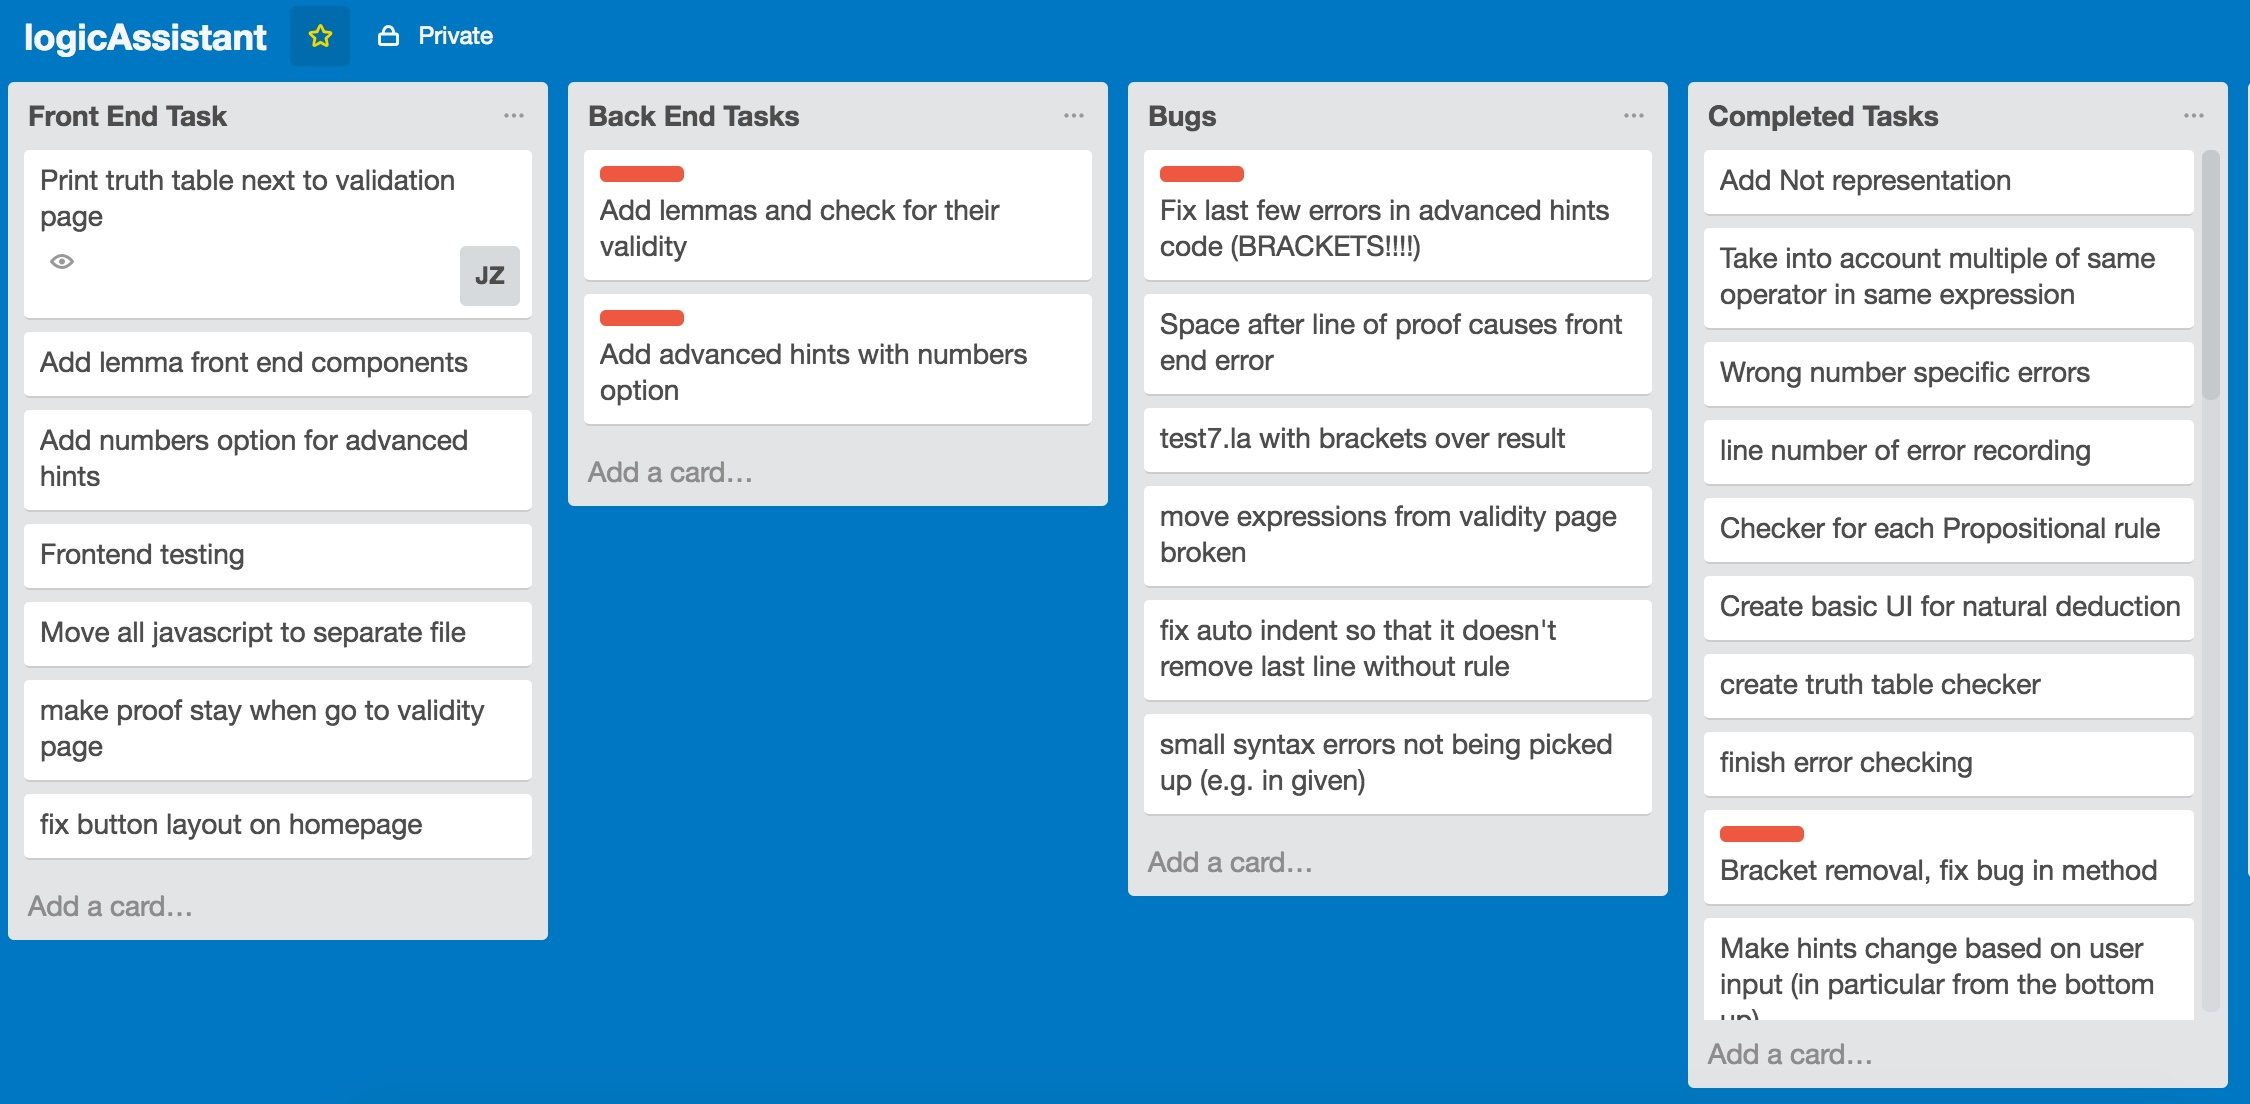
\includegraphics[width=\linewidth]{figures/trelloBoard}}
	\caption{My Trello Board}
\end{figure}

\section{Evaluation}

After carrying out a large project such as this, it is always good practise to evaluate how the project as a whole went. Were the objectives set out at the beginning of the project realistic, were you able to create all of your planned functionality, could you have avoided any set-backs that you were faced with. These ideas among others are all items to consider after having complete a project. By successfully evaluating a completed project, you will be able to use any lessons learnt to improve future projects.

\subsection{Realistic Objectives}

At the beginning of this project, I clearly set out several goals that I wanted to achieve by its completion (see \ref{objectives}). The main goals that I set out to complete were, to create a website that allows a user to type in their Natural Deduction proof and then using the functionality will be told whether their proof is valid. In addition to this I also planned to add hints that a user can request when they are stuck at any point of their proof. I also mentioned some extensions that time allowing I would also like to add such as supporting Predicate logic, saving/loading of proofs and a more advanced solving algorithm for generating hints. I felt that by completing these main objectives together with some of the extensions, I would be able to create a useful Natural Deduction tool.

In the end, I was able to successfully complete the two main objectives of the project, providing the user with an easy to use interface to help them solve their Natural Deduction problems. Once I had completed these tasks I then had to decide which features were most important for me to add. In the end I decided to add the saving and loading functionality as I realised that would make the tool much easier for the user to use. I also added a validity checker based on the premises and result of a proof, so that a user can check their proof is valid before trying to solve it. Although this was not in my list of extensions, I felt that this was a very useful tool for any user. 

The biggest decision that I had to make was whether to extend the software to be able to solve Predicate logic proofs or improve the algorithm used to generate hints. Both of these tasks would have been very time consuming, so I knew I wouldn't have enough time to do both. In the end I decided to improve hint generation, for a number of reasons. Firstly, before making this decision although a basic form of hints had been created, the methodology employed was not very useful. When the user was stuck at a point in their proof and clicked the "Hint" button,  the code would just try each of the rules and see which ones were successful. It would then output to the user which rules can be used. This is of course a very short-sighted way of doing this, that could lead a user off in the complete wrong direction. I therefore decided that hints should be perfected so that they are actually helpful for the user. If I was able to generate hints that actually help lead the user towards their specified goal, this tool would be really helping a user learn how to solve these problems. In addition to this, before moving on to a completely new logical system such as Predicate logic, where there are lots of new areas, such as quantifiers to consider, I wanted to make sure to have completely finished the functionality for Propositional logic. There would have been no point in moving on to this new logical system, if the original one had not been fully implemented. I would rather there were less features created in this project that work really well than more which work less well. Once I had made this decision I ensured to design the rest of the code-base in a way that it could be easily added to if someone were to extend it to support Predicate Logic in the future. 

Overall, I was able to complete my main objectives as well as several extensions that would make the user experience better and make this tool much more useful to the user. I think that I chose wisely when it came to choosing which extensions to complete, as in the end it has lead to a website that really can help a user who is learning how to solve Natural Deduction proofs.

\subsection{Project Plan}

At the onset of this project, I made sure to create a detailed schedule including actual dates (see \ref{schedule}), to plan the execution of this project. In each iteration I detailed what I wanted to achieve by its completion and how this would contribute towards the end product. The iterations themselves varied in length depending on how long I thought the various tasks would take to complete.

The first three iterations worked to plan with me easily being able to finish them by my specified deadlines. I was therefore by the end of iteration able to say that I had completed my main objectives together with an overall plan of how the rest of the project would be carried out. I had also even implemented some extra features that were not mentioned in the plans that I had set out. After iteration three, I had a small break in order to revise for exams. It was at this point that, as mentioned above, I decided to no longer implement Predicate Logic, but rather a more advanced hint generation system. This meant that the subsequent iterations would be slightly different. This meant that iterations four to six were merged into one as I tried to implement various proof solving algorithms and tried to solve the various bugs that I had left over from previous iterations. This was quite an intense period, but by the end I was able to complete this task. 

Although I was able to complete the tasks that I in the end decided to implement, because I changed my mind in the middle of the project, the project at points became a bit disorganised. From iteration four onwards I had no set plan of how to implement the remaining functionality which meant it was often difficult to decide what to do next. Trello (see \ref{trello}) was able to help me with this, but it still meant me wasting time trying to work out what to do next. It would have been best, you could say, for me to have planned exactly what I was going to implement at the beginning of the project. On the other hand however, it was only once I had properly started to create the main features of the software that I became aware of the choices that I would have to make due to time constraints. Before starting the project it was very difficult to estimate how long tasks would take, so I made some rough estimations when making the schedule. It was only once I actually started using this schedule that compromises had to be made. Therefore you could say I had no choice but to continue working without a plan. Although this was a small setback, I was able to complete all of the tasks that I decided were necessary.

Overall, although I chose to change the direction of the project midway I was able to complete the tasks that I decided to implement throughout this project. As a result of this I was not able to completely keep to the schedule that was set out at the beginning and should have changed the plans accordingly before continuing on with iteration four. This would have made it much easier for me to know which tasks to do when as I came towards the end of the project. I was however able to end of the project with iteration seven, where I could tidy up and finish the last parts of the important functionality that this software provides.

\subsection{Language}

\subsection{Testing}
As mentioned previously (see \ref{testing}), testing was a key component of this project as a whole. I used Test Driven Development whilst developing the back-end of the system to ensure that all parts of the system were working well as new features were added. This led to a large test-suite being created. I also created several front-end test cases which test the actual functionality that a user would utilise in order to access their required features. All of this testing greatly helped towards the carrying out of this project.

Although I was able to keep up the use of Test Driven Development for the back-end throughout the project, one could say that the amount of tests created in this area was a bit lacking. The test suite checks most of the basic cases for the various features as well as some of the edge cases. However more testing could have been done for these edge cases in order to ensure that this software works in every case. As well as this, testing was mainly carried out on relatively short proofs. This means that during the project either large proofs had to be manually tested or just assumed to work based on the smaller proof tests passing. The main reason for this was due to time constraints. Writing tests for large proofs is very time consuming and I decided to create a large number of smaller tests, which cover most of the edge cases I could think of instead. If more time was available I would spend time adding a lot more complex test-cases to this test-suite.

Another missed opportunity that I had with testing in this project was when it came to the front-end. It was only quite late into the project that I decided to add these tests. It took me a while to find an effective way to create these tests, but once I had created one successfully, I was able to easily add several more. Due to the time it took for me to work out an easy way to do this, it was not until midway through the project that I actually carried this out. This meant that in order to test the front-end of the software, I had to manually keep redeploying it. This was quite a time consuming process. Had I started to develop these tests earlier I would have been able to use them to help me with the development process itself. When I eventually created these tests I ended up deciding not to create that many of them for a number of reasons. Firstly most of the functionality had already been tested in the back-end and so had been proven to work in a lot of cases. Also the time it takes to run one of these tests is a few seconds, as they actually load the web-page and perform click and input events. This meant the test-suite as a whole would take minutes rather than seconds. It would therefore be very time consuming for me to run this test suite every time a change was made. I therefore decided to have only a limited number of these tests to prove that the front-end of this application is functioning properly.

Before starting this project, as I had done in previous projects, I considered using Continuous Integration to continuously manage the test-suite for my project. This would allow me to keep constant track of my tests and would alert me when any of them fail when subsequent features are added. This can be a very helpful tool when conducting a software project with a large set of tests like this. However, in the end I decided that I would not use a Continuous Integration tool. The main reason for this was the number of other tools that I would be using that constantly alert me to whether all of my tests are passing. Firstly, by using Intellij (see \ref{intellij}), I was provided with an easy-to-use interface for running lots of test-cases with just the click of a button. This made it easy to just run specific test-cases after a piece of code has been changed. Also by using Maven (see \ref{maven}), and in particular git hooks (see \ref{git}), I was able to run all of my tests before any changes were pushed to git, thereby ensuring that all of my code in functioning correctly. Based on the use of these two technologies, I felt that I would always be kept up to date of the health of my code, and therefore the use of Continuous Development would be unnecessary.

In summary, the testing carried out for this project was relatively thorough in the back-end, but could have been improved through an increase in testing of longer and more complex proofs. In the front-end, more tests could have also been added but a balance had to be maintained between the rigour of testing and the time they take to run. I also still agree with the premise that Continuous Integration was not necessary for this project. Despite some small short-falls, I feel that the testing I carried out through this project, greatly assisted me in its development into its completed product.

\subsection{Front-End Design}

One of the most important parts of LogicAssistant is the front-end user interface. This is the component of this application which the users themselves will be using to access the useful features, and therefore must look as good as possible. As well as being aesthetically pleasing, the front-end must also boast features which are easy to use and could be used by anyone. I therefore put a lot of thought into how I was to design the front-end of the application.

Looking back at the end design of this application, a few points can be made. Firstly, I think that the application has been created with an interface that is very easy to use. As soon as you arrive at the website you are immediately provided with the main functionality of the website, and it is immediately clear as to what the user needs to do first. All buttons are clearly labelled, with tooltips explaining certain features. This overall functionality is also quite simplistic, so that any user, no matter what their level of knowledge of this subject is, can use this application. The presence of a detailed user guide on the website also ensures that the website is as user friendly as possible. The ease of use of the user interface therefore mirrors the amount of time spent perfecting it. However, despite the large amount of time spent perfecting the front-end usability, one could argue that the design itself could be improved. When designing the website I used a very basic Bootstrap template. The reason I did this is that I felt it would be easy to add additional features to this web-page without too much of a hassle. It would also be very easy for me to make these extra features look good on the page. The entire design of the web-page could have been improved by using a better looking template in the first place. This would have made the user experience on the website even better, as it is often the design of a website that draws people into using its features. If I had more time to work on this project, this would definitely be a part of the project that I would redo, giving the web-page that slightly better aesthetic appeal.

The front-end design of this application has been created to be easy to use for users, and looks good enough to be released as a functioning website. However the overall design could still be improved, giving users an attractive website that helps them with all of their Natural Deduction proof solving needs.

\subsection{Efficiency}

In order to provide a useful service to the user, it is important that each of the features that are provided are as efficient as possible. The average user of this service will not have time to waste waiting for an algorithm to complete its processing, so the most efficient methods must be found for each feature.

\subsubsection{Proof Checking Algorithm}



\subsubsection{ND Solver Algorithm}

\subsubsection{Validity Algorithm}
use tableaux method????

\subsection{Difficulties}

Throughout my implementation of this project I was faced with a number of difficulties which hindered my overall progress. In order to solve them I had to spend large amounts of time debugging the code trying to find the route of the problem. In the end I was able to fix most of these difficulties, but a large amount of time was wasted trying to solve them.

A very large difficulty that I was faced with was when implementing the proof solving algorithm in order to generate hints. As mentioned above (see \ref{hints}), in order to generate hints for the user I implemented a proof solving algorithm to solve the proof and then based on this result generate a hint. The first problem with this was that the algorithm that I used, specified some of the Natural Deduction rules differently to how I specified them in this project. For example, for Or Elimination rather than splitting the proof into two boxes and proving the same result from each, the algorithm would prove an expression containing an Or operator and one containing the negation of one side of this Or containing expression. On top of this some rules were completely missed out of the algorithm such as all of the Only rules. In order to add in the missed in rules it was not too difficult as they followed a similar pattern to other rules. However, when it came to adding Or Elimination I had to think of a completely different method to apply this rule. This took me a very long time to perfect, wasting other time that I could have spent on adding extra features. One could argue that due to the difficulties associated with this algorithm, it may have been more beneficial for me to have used another algorithm completely. I decided not to do this because I realised that if I was able to solve the issues I would find with this algorithm, I would be able to create a very efficient way to generate hints for the user. The benefits definitely outweighed the costs, and I decided to stick with it. I was eventually able to solve these problems, thereby completing the algorithm.  

Another difficulty that I was faced with towards the beginning of this project was to do with brackets in expressions. 

Java Spring

\subsection{Competitor Comparisons}

\subsection{User Feedback}

\section{Conclusion}

\pagebreak
\appendix
\section{Natural Deduction Rules}
\label{appendix:nd}

\subsection{Propositional Rules (adapted from \cite{ndBook})}
\label{appendix:nd-prop}

\begin{namedthm}{Rule}[And Introduction]

\begin{bprooftree}
\AxiomC{$A$}
\AxiomC{$B$}
\BinaryInfC{$A \wedge B$}
\end{bprooftree}\qquad or \qquad
\begin{bprooftree}
\AxiomC{$A$}
\AxiomC{$B$}
\BinaryInfC{$B \wedge A$}
\end{bprooftree}

\end{namedthm}

\begin{namedthm}{Rule}[And Elimination]

\begin{bprooftree}
\AxiomC{$A \wedge B$}
\UnaryInfC{$A$}
\end{bprooftree}\qquad or \qquad
\begin{bprooftree}
\AxiomC{$A \wedge B$}
\UnaryInfC{$B$}
\end{bprooftree}

\end{namedthm}

\begin{namedthm}{Rule}[Or Introduction]

\begin{bprooftree}
\AxiomC{$A$}
\UnaryInfC{$A \vee B$}
\end{bprooftree}\qquad or \qquad
\begin{bprooftree}
\AxiomC{$A$}
\UnaryInfC{$B \vee A$}
\end{bprooftree}

\end{namedthm}

\begin{namedthm}{Rule}[Or Elimination]

\begin{bprooftree}
\AxiomC{$A \vdash C$}
\AxiomC{$B \vdash C$}
\AxiomC{$A \vee B$}
\TrinaryInfC{$C$}
\end{bprooftree}\qquad where A and B are assumptions

\end{namedthm}

\begin{namedthm}{Rule}[Not Introduction]

\begin{bprooftree}
\AxiomC{$A \vdash \bot$}
\UnaryInfC{$\neg A$}
\end{bprooftree}\qquad where A is an assumption

\end{namedthm}

\begin{namedthm}{Rule}[Not Elimination]

\begin{bprooftree}
\AxiomC{$\neg  A$}
\AxiomC{$A$}
\BinaryInfC{$\bot$}
\end{bprooftree}\qquad 

\end{namedthm}

\begin{namedthm}{Rule}[Double Not Elimination]
	
	\begin{bprooftree}
		\AxiomC{$\neg \neg A$}
		\UnaryInfC{$A$}
	\end{bprooftree}\qquad 
	
\end{namedthm}

\begin{namedthm}{Rule}[Implies Introduction]

\begin{bprooftree}
\AxiomC{$A \vdash B$}
\UnaryInfC{$A \Rightarrow B$}
\end{bprooftree}\qquad where A is an assumption

\end{namedthm}

\begin{namedthm}{Rule}[Implies Elimination]

\begin{bprooftree}
\AxiomC{$A$}
\AxiomC{$A \Rightarrow B$}
\BinaryInfC{$B$}
\end{bprooftree}\qquad 

\end{namedthm}

\begin{namedthm}{Rule}[Iff Introduction]

\begin{bprooftree}
\AxiomC{$A \Rightarrow B$}
\AxiomC{$B \Rightarrow A$}
\BinaryInfC{$A \Leftrightarrow B$}
\end{bprooftree}\qquad 

\end{namedthm}

\begin{namedthm}{Rule}[Iff Elimination]

\begin{bprooftree}
\AxiomC{$A \Leftrightarrow B$}
\UnaryInfC{$A \Rightarrow B$}
\end{bprooftree}\qquad or \qquad
\begin{bprooftree}
\AxiomC{$A \Leftrightarrow B$}
\UnaryInfC{$B \Rightarrow A$}
\end{bprooftree}

\end{namedthm}


\subsection{Predicate Rules}
\label{appendix:nd-pred}

\begin{namedthm}{Rule}[$\forall$ Introduction]

\begin{bprooftree}
\AxiomC{$P(a)$}
\UnaryInfC{$\forall x.P(x)$}
\end{bprooftree}\qquad where a is arbitrary \qquad

\end{namedthm}

\begin{namedthm}{Rule}[$\forall$ Elimination]

\begin{bprooftree}
\AxiomC{$\forall x.P(x)$}
\UnaryInfC{$P(a)$}
\end{bprooftree}\qquad where a is arbitrary \qquad

\end{namedthm}


\begin{namedthm}{Rule}[$\exists$ Introduction]

\begin{bprooftree}
\AxiomC{$\exists x.P(x)$}
\AxiomC{$\forall x.(P(x) \Rightarrow Q)$}
\BinaryInfC{$Q$}
\end{bprooftree}\qquad

\end{namedthm}

\begin{namedthm}{Rule}[$\exists$ Elimination]

\begin{bprooftree}
\AxiomC{$P(t)$}
\UnaryInfC{$\exists x.P(x)$}
\end{bprooftree}\qquad where t is any term

\end{namedthm}

\begin{namedthm}{Rule}[Substitution]

\begin{bprooftree}
\AxiomC{$m = n$}
\AxiomC{$S(n)$}
\BinaryInfC{$S[m/n]$}
\end{bprooftree}\qquad or \qquad
\begin{bprooftree}
\AxiomC{$m = n$}
\AxiomC{$S(m)$}
\BinaryInfC{$S[n/m]$}
\end{bprooftree}

\end{namedthm}

\pagebreak

\section{User Guide}

\pagebreak

\begin{thebibliography}{9}

\bibitem{pandora} 
Pandora (Proof Assistant for Natural Deduction using Organised Rectangular Areas) is a learning support tool designed to guide the construction of natural deduction proofs. Found at \url{https://www.doc.ic.ac.uk/pandora/}, last retrieved 7/2/2017

\bibitem{ndBook}
Software Engineering Mathematics by Jim Woodcock and Martin Loomes, 1989 edition

\bibitem{ndAlgo}
Alexander Bolotov, Vyacheslav Bocharov, Alexander Gorchakov, Vasilyi Shangin \textit{Automated First Order Natural Deduction}. Conference Paper, January 2005


\end{thebibliography}



\end{document}
